\documentclass[oneside]{stml-l}
\textheight=9in \textwidth=6in \calclayout
%\usepackage[active]{srcltx}
\usepackage{amssymb,graphicx}
%\usepackage{caption}
\usepackage[alphabetic,y2k,lite]{amsrefs}
\usepackage{multirow}
%\usepackage{overpic}
%\usepackage{pstricks}
%\usepackage{pst-node}
%\usepackage{showlabels}
%\usepackage{fancyvrb}
%%%%%%%%%%%%%%%
\renewcommand{\thesection}{\thechapter.\arabic{section}}
\numberwithin{figure}{chapter}
%%%%%%%%%%%%%%%%%%%%%%%%%%%%%%%%%%%%%%%%%%%%%%%%%%%%%%%%%%%%%%%%%%%%%
\newcommand{\apref}[1]{Appendix\ {\rm\ref{#1}}}
\newcommand{\firef}[1]{Figure\ {\rm\ref{#1}}}
\newcommand{\thref}[1]{Theorem\ {\rm\ref{#1}}}
\newcommand{\prref}[1]{Proposition\ {\rm\ref{#1}}}
\newcommand{\leref}[1]{Lemma\ {\rm\ref{#1}}}
\newcommand{\coref}[1]{Corollary\ {\rm\ref{#1}}}
\newcommand{\clref}[1]{Claim\ {\rm\ref{#1}}}
\newcommand{\conref}[1]{Conjecture\ {\rm\ref{#1}}}
\newcommand{\deref}[1]{Definition\ {\rm\ref{#1}}}
\newcommand{\exref}[1]{Example\ {\rm\ref{#1}}}
\newcommand{\ecref}[1]{Exercise\ {\rm\ref{#1}}}
\newcommand{\reref}[1]{Remark\ {\rm\ref{#1}}}
\newcommand{\quref}[1]{Question\ {\rm\ref{#1}}}
\newcommand{\seref}[1]{Section\ {\rm\ref{#1}}}
\newcommand{\chref}[1]{Chapter\ {\rm\ref{#1}}}
\newcommand{\noref}[1]{Notation\ {\rm\ref{#1}}}



%%%%%%%%%%%%%%%%%% Tikz %%%%%%%%%
%\usepackage[obeyspaces]{url}
\usepackage{amsmath,listings,graphicx}
\usepackage{hyperref,url}
% \usepackage{float}
% \floatstyle{plain}
% \newfloat{listing}{thp}{lop}[chapter]
% \floatname{listing}{Listing}

\usepackage{tikz}

\usetikzlibrary{%
  arrows,%
  shapes.misc,% wg. rounded rectangle
  shapes.arrows,%
  chains,%
  matrix,%
  positioning,% wg. " of "
  scopes,%
  decorations.pathmorphing,% /pgf/decoration/random steps ~ erste Graphik
  shadows%
}
\usetikzlibrary{calc}


%%% for warnings
\newcommand{\warningsign}%
{\raisebox{-0.7\height}{
\includegraphics[width=1.5cm]{figures/caution.pdf}}
} %

\newenvironment{warning}% 
{\begin{list}{\smash\warningsign}{%
\setlength\leftmargin{2cm}
\setlength\labelwidth{1cm}
\setlength\labelsep{1cm}
\setlength\parindent{0cm}
}
\item {\noindent\bfseries{Warning}}. }
{\end{list}}


\newcommand{\menu}[1]{{\bf\sc{#1}}}

\newcommand{\smenu}[1]{$\to$\menu{#1}}


\newtheorem*{note}{Note}


\begin{document}
\tikzset{
  global/.style={
    % The shape:
    rounded rectangle,
    % The size:
    minimum size=6mm,
    % The border:
    very thick,
    draw=blue!50!black!50,         % 50% blue and 50% black,
                                  % and that mixed with 50% white
    % The filling:
    top color=white,              % a shading that is white at the top...
    bottom color=blue!50!black!20, % and something else at the bottom
    % Font
    font=\ttfamily
  }
}
\definecolor{LightBlue1}{rgb}{.74902,.937255,1.0}
\definecolor{MistyRose1}{rgb}{1.0,.894118,.882353}

\lstset{language=C, basicstyle=\ttfamily, 
frame=single, frameround=tttt,
backgroundcolor=\color{LightBlue1}, float=p, captionpos=b,
showspaces=false, escapechar=?, escapebegin=\itshape }

%%% for code
\lstMakeShortInline~


\title[Robotics with ZumoBot]{Robotics with ZumoBot\\ {\small version 1.3, August 2016}}
\author{Alexander Kirillov}
\address{IslandBots robotic
club}
\urladdr{http://islandbots.org/}
\email{shurik179@gmail.com}
\maketitle
\thanks{
\vspace*{2in}
\noindent \centerline{
\includegraphics{figures/cc-by-nc-sa.png}}

\noindent This work is licensed under the Creative Commons
Attribution-NonCommercial-ShareAlike License.  To view a copy of this
license, visit \url{http://creativecommons.org/licenses/by-nc-sa/3.0/} or
send a letter to Creative Commons, 543 Howard Street, 5th Floor, San
Francisco, California, 94105, USA. If you distribute this work or a
derivative, include the history of the document. 

\vspace{1in}

This work is based in part on {\em Programming with Robots} by 
Albert W. Schueller, available from
\url{http://carrot.whitman.edu/Robots/}. 
}


\tableofcontents
%%%%%%%%%%%%%%%%%%%%%
\chapter*{Introduction}
These notes contain a short introduction to programming Zumo 32U4 robot, produced by Pololu, using 
Arduino IDE. It is intended for people with little to none programming experience.  

It was originally written for  {\sl SigmaCamp}
(\url{http://sigmacamp.org}),  a science summer camp where the author was
teaching a course on robotics, and for members of {\sl IslandBots} robotics
club (\url{http://islandbots.org}), of which the author is the coach. 


If you have any  comments, suggestions, or corrections, please send them
to {\texttt shurik179@gmail.com}. 

%%%%%%%%%%%%%%%%%%%%%
\chapter{Introducing Zumo robot}
Zumo 32U4 is a small tracked robot, manufactured  and sold by Pololu:
\url{https://www.pololu.com/product/3124}. At the heart of the robot is 
ATmega32U4 microcontroller, which can be programmed using a very
 popular Arduino IDE (integrated development environment), essentially 
 a version of C++ programming language. The robot is equipped with two motors, 
 a small LCD screen, and a variety of sensors. 
 \begin{figure}[ht]
 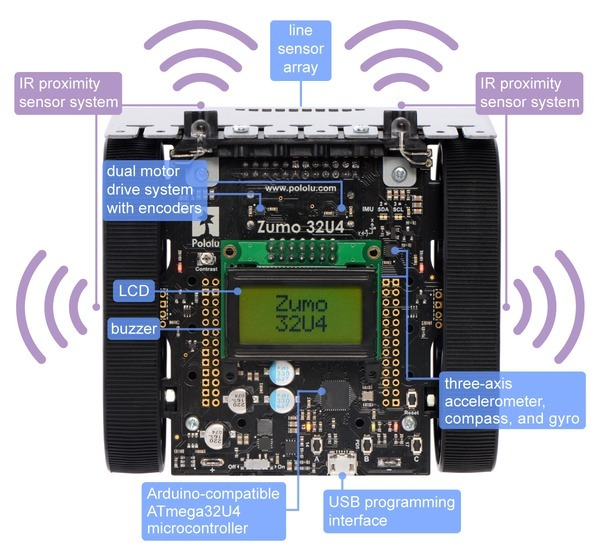
\includegraphics[height=10cm]{figures/zumo-overview.jpg}
 \end{figure}

The robot runs on 4 AA batteries; to program it, you need to connect it to a 
computer using a microUSB cable (the same cable  used by Android cell phones). 
Detailed description of Zumo robot is given in the user guide on Pololu website:
\url{https://www.pololu.com/docs/0J63}.


%%%%%%%%%%%%%%%%%%%%%
\chapter{Hello, world!}
In this chapter, we run our first program for the Zumo Bot. Our instructions 
assume that you are  using a recent version of Windows operating system 
(Windоws 7 or above). You can also program Zumo on  Mac or Linux; check  
Pololu website for instructions.
\section{Installing the software}
First, you need to install Arduino IDE. It is freely available on Arduino 
website: \url{http://arduino.cc}. The installation is straightforward; 
if you have any difficulties, check the instructions on the website. 
If you already have Arduino installed, make sure you have a recent version 
(at least 1.6.2). 

Next, you need to install the custom library for Zumo, created by Pololu. 
To do that:
\begin{itemize}
\item In the Arduino IDE, open in the menu 
         \menu{Sketch}\smenu{Include Library}\smenu{Manage Libraries...}.
\item Search for ``Zumo32U4''.
\item Click the Zumo32U4 entry in the list.
\item Click ``Install''.
\end{itemize}

You will also  need to install the custom drivers and board definitions for 
Zumo (not necessary but advised under Windows 10; required for previous 
versions of Windows).  To do this:
\begin{itemize}
\item Download the zip file from Pololu website: 
\url{https://www.pololu.com/file/download/a-star-2.0.0.zip?file_id=0J743}
\item Extract it to a temporary location
\item Inside the extracted folder, find subfolder ~drivers~. Right-click 
on the file ~a-star.inf~ and select ``Install'' from the pop-up menu. The 
installation normally only takes several seconds.  In case of any errors, 
check Zumo User guide, Section 5.1, \url{https://www.pololu.com/docs/0J63/5.1}, 
for more detalis. If you do not get any error messages, it means that 
the installation was successful.  
\item 
Copy the ~pololu~ folder from the downloaded ~add-on~ folder into 
the ~[sketchbook location]\hardware~ folder, where ~[sketchbook location]~ 
is the directory where your arduino sketches are. Normally it would be    
~C:\Users\<username>\Documents\Arduino\hardware\pololu~

If the ~Arduino~ or ~hardware~ directories do not exist yet, you  need 
to create them.

\end{itemize}

\section{Uploading and running programs}
You are now ready to upload your first program to Zumo. Start Arduino IDE; 
it opens an empty program (``sketch''). Ignore it and select in the menu
 \menu{File}\smenu{Examples}\smenu{Zumo32U4}\smenu{BlinkLEDs}. This loads 
a simple example program,  which blinks  Zumo's built-in LEDs. This program 
is part  of Zumo 32U4 library. Read the program and comments 
to see how it works; even if you are not familiar with these commands, 
their meaning is easy to guess. 

Connect Zumo to the computer using a micro USB cable (it is not necessary 
to turn Zumo on --- USB cable  provides the required power). Select in Arduino 
IDE menu \menu{Tools}\smenu{Board}\smenu{Pololu A-star 32U4}. 
After that, go to \menu{Tools}\smenu{Port} and select the port which has 
``Pololu 32U4'' next to it.  (The board choice is remembered, so you only 
need to do it once; the port might change every time you reconnect Zumo.)



Now, click on ``Upload'' icon (a circle with green arrow pointing to the 
right, immediately under \menu{File} menu). If everything works as expected, 
some messages will scroll in the bottom area of the window. Wait until you 
see message ``Upload complete'' in the green strip between the main part 
with program code and the bottom part, where the messages were displayed. 
If you see it, you have successfully uploaded your first program --- and 
it should immediately start working, blinking the LEDs. You  now can  
disconnect Zumo from the computer; the program you uploaded is on it and 
it will automatically start working every time you turn Zumo on. 

\section{Help and troubleshooting}
A description of the basics of Arduino programming is given  in \chref{c:arduino}. 
You can also use Arduino IDE's built-in help (under \menu{Help} menu item); 
in particular, \menu{Help}\smenu{Reference} describes many of the basic 
functions and  structures of Arduino IDE. 

Installation of Zumo 32U4 library for Arduino is covered in {\em Zumo User Guide} 
\url{https://www.pololu.com/docs/0J63/5.1}. The library itself is fully 
documented here: 
\url{http://pololu.github.io/zumo-32u4-arduino-library/index.html}.
%%%%%%%%%%%%%%%%%%%%%
\chapter{Robot motion}
We are now ready to start programming the robot. To make it easier, we 
will be using a set of custom functions, written by Alexander Kirillov, 
which are slightly more user-friendly than the original Zumo32U4 library. 

\section{First example}
Download and extract the zip file ~ZumoBot-Shurik~. Navigate to the 
extracted folder; you will see there the files ~ZumoShurik.cpp~, ~ZumoShurik.h~, 
and ~ZumoBot.ino~. The first two files contain the custom functions; 
the last file is an example of a program using these functions. 
Click on  ~ZumoBot.ino~ to open it in Arduino IDE; it should look like this. 

\begin{lstlisting}
#include <Wire.h>
#include <Zumo32U4.h>
#include "ZumoShurik.h"
void setup() {
    // put your setup code here, to run once:
    printLcd("Press A'', "to start'');
    // wait until user presses button A
    buttonA.waitForButton();
}

void loop() {
  // put your main code here, to run repeatedly: 
  // go forward for 400mm=40cm
  goForward(400);
  // turn right 90 degrees
  turn(90);
  beep(400); //produce a beep with frequency 400 hz
  delay(1000); //wait for 1000ms=1 sec
}
\end{lstlisting}

The first two lines load required libraries. Line ~#include "ZumoShurik.h"~ 
loads files ~ZumoShurik.h~ and ~ZumoShurik.cpp~. Both of these files must 
be in the same directory as the Arduino sketch; if you are writing your 
own program, make sure to copy these files into the program directory. 
An easy way to do it is to open the example program and then use 
\menu{File}\smenu{Save As}; this will create a copy of the example file 
and of the files ~ZumoShurik.h~ and ~ZumoShurik.cpp~.

You can upload the example file and run it to see how it works. 

\section{Buttons and LCD}

Zumo provides several options for interacting with the user. It has a 
small 2-line LCD display (up to 8 symbols on each line), several LEDs, and three 
buttons labelled A, B, and C (the buttons are tiny). In addition, it has a built-in buzzer.


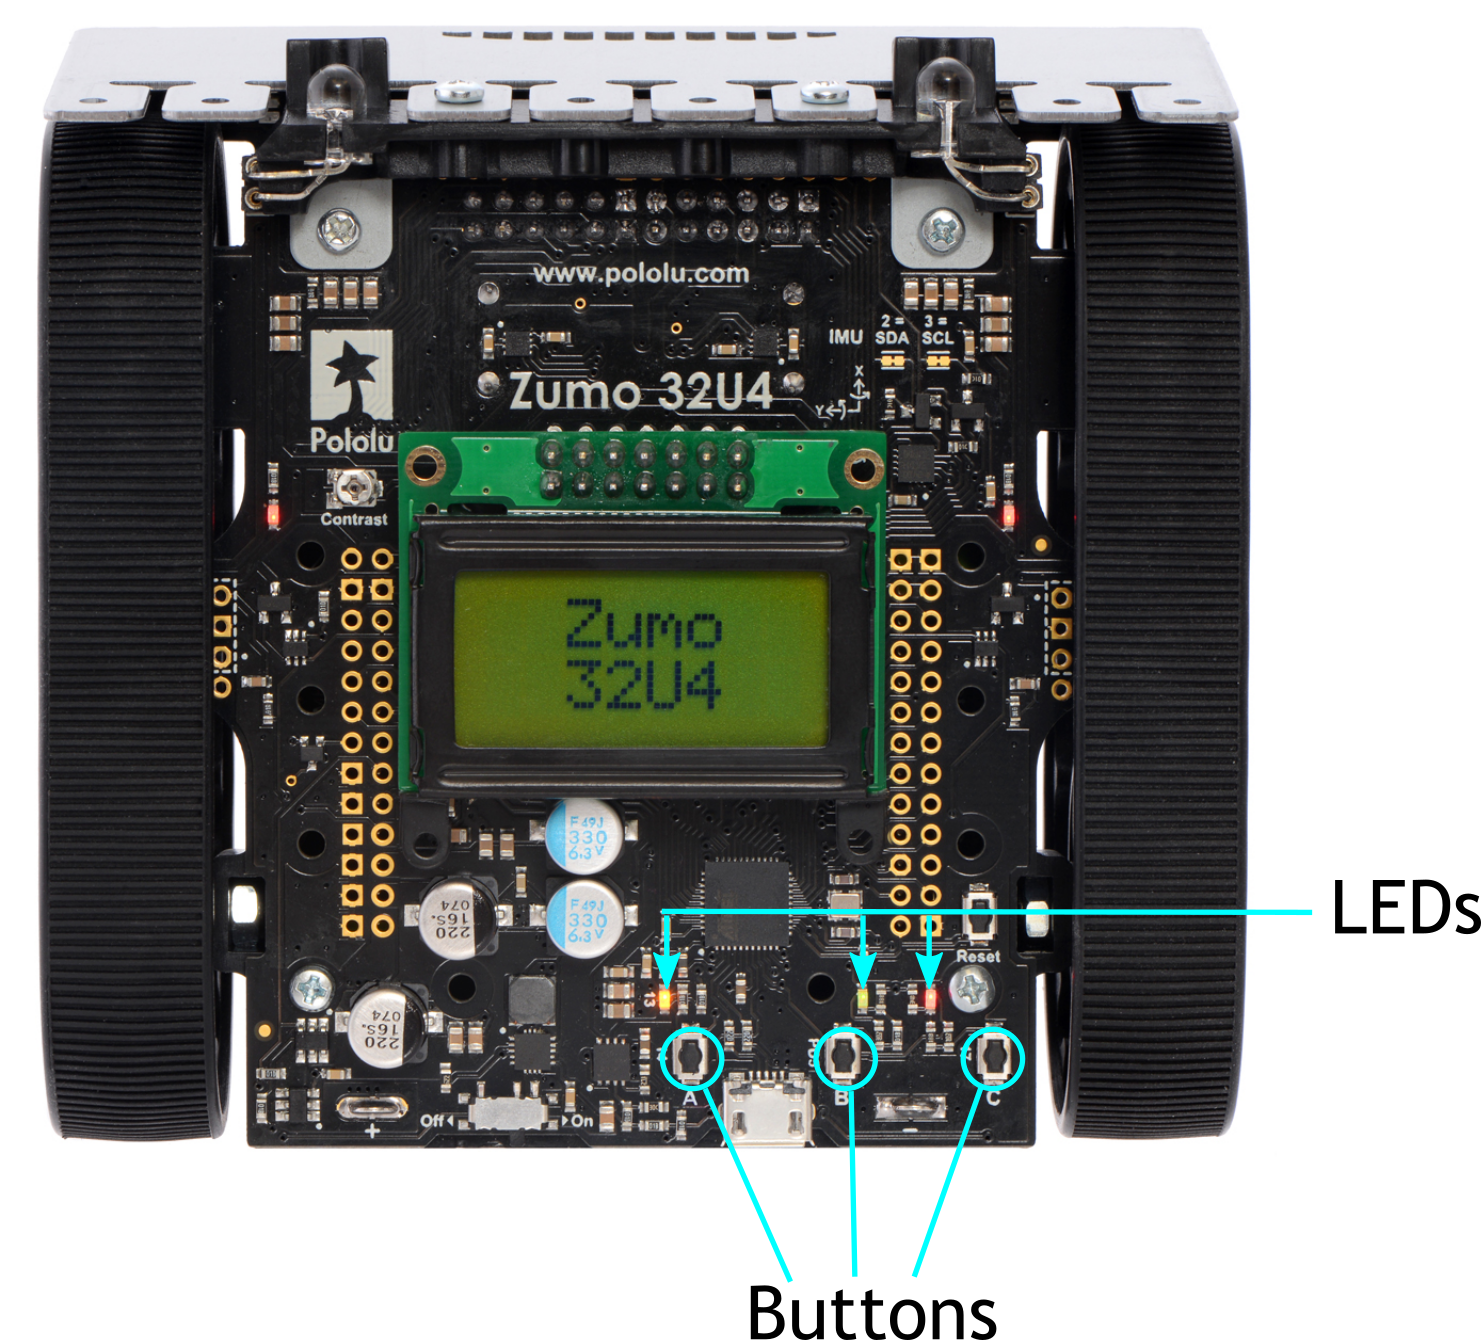
\includegraphics[height=8cm]{figures/buttons.png}

Below are the most useful commands for controlling these elements; 
all of these commands are available once you have included ~Zumo32U4.h~ and 
~ZumoShurik.h~. In this table, as in all the tables that follow, the first column
shows the type of value returned by the function. If the function does not 
return any value, the first column shows ~void~.

\begin{tabular}{|l | l | p{7cm}|}
\hline 
void & ~printLcd(String s1, String s2)~ & Prints the two strings to LCD, 
        as line 1 and line 2. Note that each LCD line can only show 8 symbols.\\ 
\hline
void & ~buttonA.waitForButton()~ & Pause program execution 
                      until the button  is pressed and released.\\ 
\cline{1-2}
void & ~buttonB.waitForButton()~& \\
\cline{1-2}
void & ~buttonC.waitForButton()~& \\
\hline
void & ~ledGreen(bool on)~ & Turns LED on/off. Use on=true or 1 to turn on, 
                              false or 0 to turn off.\\ 
\cline{1-2}
void & ~ledYellow(bool on)~& \\
\cline{1-2}
void & ~ledRed(bool on)~& \\
\hline
void & ~beep(int frequency, int duration=500)~& produces a beep of specified 
frequency (in Hz) and duration (in milliseconds). Duration is optional; if omitted, 
defaults to 500 ms=0.5 sec. For frequency, good choice woudl be values of 400--2000.
\\
\hline
\end{tabular}

For playing beeps, please note that the program does not wait for the sound to complete: 
program execution continues while the sound is playing. 


\section{Motor control}

The robot has two motors, both equipped with encoders, or rotation counters. 
The encoders can be used to compute the distance travelled or stop the robot 
once we have travelled certain distance. To turn, we run the motors in 
opposite directions. 

Below is the list of commands for controlling robot motion.
 
\par\noindent
\begin{tabular}{|l | l | p{7cm}|}
\hline 
~void~ & ~goForward(long distance, int speed=70)~ & Go forward/backward 
             for specified distance, in mm. Distance must always be positive. 
             Optional parameter ~speed~ determines speed (must be between 0-100); 
             if it is omitted, default value of 70 is used.
\\
\cline{1-2}
~void~ & ~goBackward(long distance, int speed=70)~ & \\
\hline
~void~ & ~turn(int angle, int speed=70)~ & Turn by specified angle (in degrees). 
                  Positive angle gives clockwise rotation, negative gives counterclockwise 
                  rotation. Optional parameter ~speed~ determines speed 
                  (must be between 0-100).
\\
\hline
~void~ &~setMotors(int left, int right)~ & Set the speed of both motors. 
                     Speed of each must be between -100 and 100.  \\
\hline
~void~ &~stopMotors()~ & Self-explanatory\\
\hline
~void~ &~resetEncoders()~ & Resets the encoders (rotation counters) on both motors. 
                      Note that encoders are also reset when you 
                      use ~goForward()~, ~goBackward()~. \\
\hline
~int~ & ~distanceTraveled()~& Returns distance travelled since the last 
                encoder reset, in mm. Distance is computed by using the average 
                of both motor encoders. Negative distance corresponds to motion backward. \\
\hline
~int~ & ~angleTurned()~& Returns the angle by which the robot has turned  since the last 
                encoder reset, in degrees (positive values for clockwise). Angle  is computed  
                using the difference of  motor encoders and is not very precise.  \\
\hline
\end{tabular}

Parameter ~speed~ used by ~goForward~ and  ~goBackward~ is expected to be 
between 0-100. Values larger than 100 are allowed, but give the same result as the 
value of 100. Similarly, for ~setMotors~, each of the speeds can be lower than -100 
or higher than 100, but it gives the same result as value of -100 or 100 respectively. 

%%%%%%%%%%%%%%%%%%%%%
\chapter{Using sensors}

In this section, we describe how one uses the sensors provided by Zumo. 

\section{Front sensor array}
Zumo contains an array of five infrared reflected light sensors, 
which are attached at the front of the robot pointing down (see 
\firef{f:front_array}). They are named DN1 through DN5, with DN1 being the 
leftmost.

\begin{figure}[ht]
\includegraphics[height=8cm]{figures/array.png}
\caption{Front sensor array}\label{f:front_array}
\end{figure}
Each sensor combines an infrared LED aimed down, and a 
photosensitive element, which is used to measure the intensity 
of reflected light. This allows one to determine how dark the 
floor is. We will only be using it in the situation when the 
floor is white, with some black markings, or vice versa (which is 
a common setup for robotics: black line on white surface could be 
used as a line to be followed, or as border of the field, or as 
walls of a maze). 

Zumo can be configured in two different ways: 
\begin{itemize}
\item All five front sensors are active (but then some of the 
proximity sensors, described in the next section, will be disabled)
\item Only three front sensors are active (DN1, DN3, DN5), and all 
proximity sensors are active.
\end{itemize}
To switch from one configuration to another, you need to physically 
move jumpers on the front sensor array; see Section 3.5 in 
{\it Zumo User Guide} for details. 

Before using sensors, one needs to activate and calibrate them.  
To do that, use function ~calibrateSensors(mode)~, provided by 
~ZumoShurik~ package. This should be done in the ~setup~ function 
of the sketch. Allowed values for argument ~mode~ are ~LINEARRAY~ 
(if using the configuration when all five sensors of the front 
array are active) or ~PROXIMITY~ (if only three sensors of the 
front array are active). These values should be entered without 
quotes --- these are predefined constants, not strings. 

 For calibration, the robot will turn 360 degrees in place, all 
 the time recording the sensor readings. The lowest reading will 
 be interpreted as black level, and the highest as the white level. 
 Thus, before running this function, a robot must be placed so that 
 when rotating, it would see both white and black (e.g., on top of 
 a white line). It is also advised that you put ~buttonA.waitForButton()~ 
 before and after the calibration function, to make it easier to 
 place the robot in the required starting position. 
 
After the calibration, you can read the sensor values using the 
functions below.

%%%%%%%%%%%%%%%%%%%%%%%%%%%%%%%%%%%%%%%%%%%%%%%%%%%%%%%%%%%%%%%%%%%%%%
 \noindent\begin{tabular}{|l | l | p{7cm}|}
\hline 
void & ~calibrateSensors(mode)~ & Calibrates line and proximity sensors, 
         by having the robot rotate 360 degrees and determining the 
         highest and lowest value.   Allowed values for ~mode~ are 
         ~LINEARRAY~ and ~PROXIMITY~ .\\ 
\hline
void & ~readLineSensors()~ & Reads the values of line sensors 
              (they are saved in an internal variable, which you rarely 
              need to use directly.)\\ 
\hline
boolean & ~sensorOnWhite(sensorNum)~ & Checks whether given front 
                sensor is on white/black. Allowed values of ~sensorNum~ are 
                DN1 through DN5.  See warning below.\\
\cline{1-2}
boolean & ~sensorOnBlack(sensorNum)~ &\\
\hline 
boolean &~allOnWhite()~ & Are all sensors on white? (See warning below.)\\
\hline
boolean &~allOnBlack()~ & Are all sensors on black? (See warning below.)\\
\hline

\hline
int &~linePosition()~& 
     Checks the values of all five sensors and returns the position 
     of the white line under the robot.  Returns number between -100 
     (line all the way to the left of the robot) and 100 (line all 
     the way to the right). Value 0 shows that the robot is centered 
     on the line. \\
 \hline

\end{tabular}
%%%%%%%%%%%%%%%%%%%%%%%%%%%%%%%%%%%%%%%%%%%%%%%%%%%%%%%%%%%%%%%%%%%%%%%%%

\medskip
\begin{warning}
For performance reasons, getting the values of the sensors is a 
two-step process: first you call function ~readLineSensors()~, which 
reads all the sensor values at once and saves them. After this, you 
can use functions ~sensorOnWhite()~, etc, which use the sensor values 
obtained at last reading. Thus, to get accurate results, function 
~readLineSensors()~ must be called shortly before calling functions 
~sensorOnBlack()~ and other functions in the list above. It is a good 
idea to put ~readLineSensors()~ function in the beginning of each ~loop()~. 
\end{warning}


Notes: 
\begin{enumerate}
\item The cutoff value used to distinguish between black and white 
is set in file ~ZumoShurik.cpp~. In most cases the default value 
should work fine, but if you need to change it, search this file 
for ~LIGHT_THRESHOLD~ and change the value as required. 

\item Functions ~allOnBlack()~, ~allOnWhite()~ work in both configurations; 
in the configuration where only three front sensors are active, they 
only check the values of these three. 

\item Function ~linePosition()~ assumes the white line on 
black background. It only works in five sensor configuration, and 
to work reliably, the white line should be at least 3/4 inch wide 
(standard masking tape, which is 0.94'' wide, works well). 

\end{enumerate}
 
 Below is a sample program using sensors. This program would have 
 the robot moving forward until at least one of the sensors sees white. 
 
 
 \begin{lstlisting}
#include <Wire.h>
#include <Zumo32U4.h>
#include "ZumoShurik.h"
void setup() {
    printLcd("Press A", "to start");
    buttonA.waitForButton();
    //calibrate the sensors, in 5 sensor mode
    calibrateSensors(LINEARRAY);
    printLcd("Done", "Press B");
    buttonB.waitForButton();
}

void loop() {
    readLineSensors();
    if (allOnBlack()) {
       //start going forward, at 70% speed
        setMotors(70,70);
    } else {
        //stop
        stopMotors();
        beep(400);
    }   
}
\end{lstlisting}
 
 
\section{Proximity sensors}
Zumo provides several proximity sensors. These sensors combine an 
infrared LED, which sends pulses of IR light, and IR photosensitive elements, 
which react to the reflected light. To prevent photosensitive elements 
from reacting to IR light from other sources, Zumo uses modulated 
IR light: the receivers only react to the IR light at certain frequency. 

These sensors are short-range; exact range depends on the object 
being detected, its size,  and reflectivity (in IR light). Typical range 
is about 15-20 cm. 

Due to technical constraints, these sensors do not give the distance 
to the object;  the return value is determined in a more complicated way. 
However, the basic rule stays the same:  the higher the return value, 
the stronger the reflected light, and thus, the closer is the object. 

Zumo has four IR LEDs used for proximity sensors (left, right, front left, 
front right) and three IR receivers: the front IR receiver (hidden behind 
the blade) is used to detect the reflected light  from front left and 
front right IR LEDs. For more technical details, check {\it Zumo User Guide}. 

In the ~LINEARRAY~ configuration, when all five sensors of the front line 
array are active, only the left front and right front IR LEDs (together 
with the front receiver) are active. In the ~PROXIMITY~ configuration, 
when only 3 sensors of the front line array are active, all proximity 
LEDs and receivers are active. 

To access the readings of proximity sensors, use the functions below.


 \noindent\begin{tabular}{|l | l | p{7cm}|}
\hline 
void & ~calibrateSensors(mode)~ & Calibrates line and proximity sensors.  
 Allowed values for ~mode~ are ~LINEARRAY~ and ~PROXIMITY~ .\\ 
\hline
void & ~readProxSensors()~ & Reads the values of proximity sensors 
                             (they are saved in  an internal variable, 
                             which you rarely need to use directly.)\\ 
\hline
int & ~proxSensorLevel(sensorNum)~ &
                          Returns the reading of a given proximity sensor. 
                          Allowed values of ~sensorNum~ are ~PROX_L~ (left),
                          ~PROX_LF~ (left front),  ~PROX_RF~  (right front), 
                          ~PROX_R~ (right).  Returned values can be 0--6; 
                          the higher the value, the stronger the reflected light. 
                           See warning below.\\
 \hline
\end{tabular}
%%%%%%%%%%%%%%%%%%%%%%%%%%%%%%%%%%%%%%%%%%%%%%%%%%%%%%%%%%%%%%%

\medskip
\begin{warning}
For performance reasons, getting the values of the sensors is 
a two-step process: first you call the function ~readLProxSensors()~, 
which reads all the sensor values at once and saves them. Note 
that this function takes significant time (about 15ms). After this, 
you can use functions ~proxSensorLevel()~, which use the sensor 
values obtained at last reading. Thus, to get accurate results, 
function ~readProxSensors()~ must be called frequently enough. 
It is a good idea to put this function in the beginning of each ~loop()~. 
\end{warning}





%%%%%%%%%%%%%%%%%%%%%
\chapter{Project 1: line follower}
In this chapter, we do our first project: a robot that
follows a line on the floor. We will make a line by putting 1-inch wide
white masking tape on a black surface (a sheet of plywood painted black).
You can make your own field; just make sure the line is at least one inch
wide and doesn't have sharp turns.

Before we start writing code, we need to describe the algorithm the robot
will be using --- first in human language, then translate it to C++.  

The obvious algorithm is ``start on the line; go forward until you get off
the line; turn to get back on the
line; repeat''. 

However, this algorithm will result in very jerky movement: the robot 
will only start correcting its course when it gets completely off the line. 
Since we have a whole array of front line sensors, we can use them 
to detect even small deviation from the right course --- when the robot is still
on the line, but the line is not exactly under the center of the robot --- and start
correcting before we get off the line. To correct, we would be going forward but 
steering more to the left or right as needed: if the line is to the left of the robot 
center, we must be steering left; if the line is to the right, we must be steering right.  

This leads to the following algorithm 
\begin{lstlisting}
loop(){
    ?get the line position? 
    ?go forward steering left or right as needed to correct the position?
}
\end{lstlisting}

Note that here we are continuously correcting our steering using the sensor 
feedback.  To translate this algorithm to an actual program, we need to 
explain how one steers left or right.  This is easy: to have the robot
steer to the right, we need left motor to have more power than the right. 
Thus, the command would be ~setMotors(70+correction, 70-correction)~. 
It makes sense to have the parameter ~correction~  proportional to the 
difference between the actual line position and the desried one: the 
farther off we are,  the more we need to turn.  

This gives the following program 
\begin{lstlisting}
float Kp=1.5;
loop(){
    readLineSensors();
    int error=linePosition();
    setMotors(70+Kp*error, 70-Kp*error);
  }
\end{lstlisting}
Double-check the sign: if ~error~ is negative (line to the left), we need to 
be steering left, so the left motor should have less  power than the right; 
if ~error~ is positive, we will be steering right. 

The value of the coefficient ~Kp=1.5~ was chosen so that when the line is 
all the way to one side (error=100), the motors will be given power 
$70+150=220$, $70-150=-80$. Since the motor power can't be more than a 100, 
the actual values would be $100, -80$, so the robot will be essentially 
turning in place. 

You can test what happens if $1.5$ is replaced by another value. If the 
value is too large, the robot will turn very quickly even for small 
errors, which can lead to the robot spending most time turning left 
and right, with very little headway. If the value is too small, the 
robot will be turning very little, which can cause it to miss a sharp 
turn. You can experiment to find the best value. 

The same idea of correcting the course using sensor feedback, with 
the correction proportional to the error, can be used in many 
other situations. Instead of following the line, we could use it 
to turn to  face an obstacle (using front proximity sensors), or 
face up on an inclined surface, or many other similar situations. 

%%%%%%%%%%%%%%%%%%%%%
\chapter{Project 2: Maze Solver}
\section{Description of the challenge.} The maze is made of
approx. $3\times 5$ ft sheet of plywood, painted black. 
White masking tape (0.94 in wide) is used to mark passages 
forming the maze; these lines follow rectangular grid with 
0.5 ft squares. 


\begin{tikzpicture}
\coordinate (A) at (0,0);
\coordinate (B) at (0, 6);
\coordinate (C) at (10, 6);
\coordinate (D) at (10, 0);
\draw [fill=black] (A) rectangle (C);
\draw [line width=2pt, black!80, step=1cm] (A) grid (C);
\draw [line width=2pt, white] (0,1)--(2,1)--(2,3);
\draw [line width=2pt, white] (1,3)--(3,3);
\draw [line width=2pt, white] (1,2)--(1,5)--(4,5)--(4,2);
\draw [line width=2pt, white] (3,4)--(3,1)--(9,1)--(9,2)--(5,2)--(5,4)--(3,4);    
\draw [line width=2pt, white] (7,2)--(7,3);
\draw [line width=2pt, white] (8,3)--(6,3)--(6,5)--(9,5);
\draw [line width=2pt, white] (9,1)--(9,4);
\draw [line width=2pt, white] (7,4)--(10,4);
\end{tikzpicture}

The goal is  programming a robot to find its way out of the
maze, using one of the  algorithms described below.


\section{Wall  following algorithm: simplified version}
The simplest algorthm for solving the maze is the wall following algorithm:
\begin{quote}
  Start following passages, and whenever 
you reach a junction always follow the  leftmost open passage. This 
is  equivalent to a human walking in the  a maze by putting his 
hand on the left wall and keeping it on the wall as he walks through. 
\end{quote}
This method  is guaranteed to find an exit if we start at the entrance 
to the maze; then  this method allows us to explore a section 
of the maze and find our way out. However, it  is not guaranteed to 
find an exit if we start in the middle of the maze: the robot could be 
going in circles around an ``island'' inside the maze.

The first draft of the program looks as follows (not including ~void setup()~ function):
\begin{lstlisting}
boolean passageLeft;
int speed;
void loop (){ 
    goToIntersection();
    checkIntersection();
    ?if there is a passage to the left, turn left; otherwise do nothing?
}
\end{lstlisting}
Function ~goToIntersection()~ should follow the line until we reach an 
intersection. 

Function ~checkIntersection()~ should do two things: 
\begin{itemize}
\item Move forward so that the center (not front!)  of the robot is 
above the intersection. 
\item While doing this, check whether there is a passage to the left 
and set variable ~passageLeft~
\end{itemize}

We can now fill in the details:
\begin{lstlisting}
void goToIntersection(){
    boolean atIntersection=false;
    float Kp=1.5;
    
    while (!atIntersection) {
        readLineSensors();
        setMotors(speed+Kp*linePosition(), 
                  speed-Kp*linePosition());       
        atIntersection=sensorOnWhite(DM1) || sensorOnWhite(DM5); 
    }//end of while loop
    stopMotors();
}    
\end{lstlisting}

For function ~checkIntersection()~, we will be going forward until 
we have travelled 5 cm;  while doing this, we will be checking the 
line sensors. If the leftmost line sensor (DM1)  sees white, we set 
variable ~passageLeft~ true. (Also, we should remember to set it 
to ~false~ initially):
\begin{lstlisting}
void goToIntersection(){
    passageLeft=false;
    resetEncoders();
    setMotors(speed,speed);
    while (distanceTraveled()<50) {
          readLineSensors();
          if (sensorOnWhite(DM1)) {
              passageLeft=true;
          }
    }
    stopMotors();
}
\end{lstlisting}

Now, all that remains to do is write the piece of code implementing 
instruction \\
~ if there is a passage to the left, turn left; otherwise do nothing~, \\
which is straightforward. 

\section{Wall following: the full version}
The algorithm described in the previous section has obvious deficiencies. 
First, it only checks  for open passage to the left. Correct algorithm 
should check for open passages to left, right, 
and front, and turn accordingly.

Second, the function ~goToIntersection~ detects the intersection by 
using two light sensors,  leftmost and rightmost. Thus, it would be 
unable to detect a dead end.

To fix the first issue, we introduce two more boolean global variables, 
~passageRight~ and  ~passageForward~, and modify the function ~checkIntersection~ 
accordingly. The proper  way to detect existence of forward passage should 
be by checking whether one of the three sensors DM2, DM3, DM4 sees white 
after we move forward by 5 cm (not during move!). 

The second issue is fixed by replacing line 

~ atIntersection=sensorOnWhite(DM1) || sensorOnWhite(DM5); ~

with 

~ atIntersection=sensorOnWhite(DM1) || sensorOnWhite(DM5) || allOnBlack(); ~

Finally, the logic determining where to turn should be different. Namely, it should be 
\begin{lstlisting}
if (passageLeft) {
    turn(-90);
} else if (passageForward) {
   //do nothing
} else if (passageRight) {
    turn(90);
} else {
   // no open passages left, front, or right
   turn(180);
}
\end{lstlisting}

We leave it to the reader to write the full program. 
 
 \section{Pledge algorithm}
This is a modified version of wall following that's able to 
jump between islands, to solve mazes wall following can't. 
It's a guaranteed way to reach an exit on the outer edge 
of any 2D maze from any point in the middle.  However, 
it is not guaranteed to visit every passage inside the maze, 
so this algorithm will not help you if you are looking 
for a hidden treasure inside the maze. 

\begin{quote}
Start by picking a direction, and always move in that 
direction when possible. When you  hit a wall, start wall 
following, using the left hand rule.  When wall following, 
count the number of turns you make, e.g. a left turn is -1
 and a right turn is 1. Continue wall following until your 
 chosen direction is available again {\bf and} the total 
 number of turns you've made is 0; then stop following wall 
 and go in the chosen direction until you hit a wall. Repeat 
 until you find an exit. 
\end{quote}

Note: if your chosen direction is available but  the total 
number of turns is not zero (i.e. if you've turned around 360 
degrees or more), keep wall following until you untwist yourself. 
Note that Pledge algorithm may make you visit a passage or the 
start more than once, although subsequent times will always be 
with different turn totals.

The figure below illustrates this method:

\begin{tikzpicture}
\draw[help lines] (0,0) grid[step=0.5] (7,5);
\draw[line width=4pt] (1,4) -- (6,4) -- (6,1)--(3,1)--(3,2.5)--(4,2.5);
\draw[very thick, red, ->](0,3.5)-- (1, 3.5);
\draw[very thick, red, ->](1,3.5)-- (5.5, 3.5)--(5.5, 1.5)
     --(3.5, 1.5)--(3.5,2)--(4.5,2)
     --(4.5, 3)--(2.5,3) -- (2.5,0.5) --(7,0.5);
\node[circle,draw=blue!50,fill=blue!20,thick, inner sep=1pt] 
         at (3.5, 2) {$1$};
\node[circle,draw=blue!50,fill=blue!20,thick, inner sep=1pt] 
         at (2.5, 0.5) {$2$};
\end{tikzpicture}

Thick black lines show the walls of the maze; the red line shows 
the path of the robot. At point 1, robot turns to so that it is  
again heading the same direction as in the beginning; however, the 
number of turns at this point is not zero, so the robot continues 
following the wall. At point 2, the robot is again heading in the 
original direction, and the number of turns is zero, so it stops 
following the wall. Had the robot left the wall at point 1, it would 
be running in circles.   


\section{Coding Pledge algorithm}
To program Pledge algorithm, we need to keep track of robot direction
and number of turns. In fact, just the number of turns is sufficient: if we 
know the number of turns, we can determine the direction. Thus, we introduce 
a global variable ~numTurns~. Every time we turn 90 clockwise, ~numTurns~ 
is increased by 1;  every time we turn 90 degrees counterclockwise, we decrease 
~numTurns~ by  1. 

Thus, the draft of the program would be 
\begin{lstlisting}
int numTurns=0;
void loop(){
    goToWall();
    followWall();    
}
\end{lstlisting}
where
\begin{itemize}
\item Function ~goToWall()~ goes forward along the line, through 
intersections, until the robot hits a wall
\item Function ~followWall()~ follows the wall using left hand rule 
until we are again facing the same direction as before, with ~numTurns=0~.
\end{itemize}

For each of  these functions, we need to describe carefully what 
conditions the function expects at the start and in what condition 
it leaves the robot at the end (which way is it facing? is it at intersection?)

For ~goToWall()~:

\begin{itemize}
\item Initial condition: robot is on the line (i.e., the line is under the 
center of the front sensor array; robot could be at intersection), ~numTurns=0~
\item Final state: robot is at an intersection, there is a wall ahead 
(i.e., no passage forward), and  ~numTurns=0~
\end{itemize}

For ~followWall()~:
\begin{itemize}
\item Initial condition: robot is at an intersection, there is a wall ahead 
(i.e., no passage forward), and  ~numTurns=0~
\item Final state: robot is on the line (i.e., the line is under the 
sensor of the front sensor array; robot could be at intersection), ~numTurns=0~
\end{itemize}

When we think about implementing the algorithm, we see that in the 
very beginning of ~followWall()~, the robot needs to turn so that the wall 
is on its left. Normally it would be just a 90 degree right  turn; however, 
if we are at a dead end, we need to turn 180 degrees. Thus, we need to know 
whether there is  a passage to the right. Therefore, we add one more 
condition to the final state of ~goToWall()~:
\begin{itemize}
\item Final state: robot is at the intersection, there is a wall ahead 
(i.e., no passage forward),  ~numTurns=0~, and global variable 
~passageRight~ contains information about whether there is a passage to the right. 
 \end{itemize}
 
 To implement these two functions, we will make use of the functions 
 ~goToIntersection()~, ~checkIntersection()~ which we used for 
 wall-following algorithm. Implementing ~goToWall()~ is trivial; for 
 ~followWall()~, in the beginning we must put 
 \begin{lstlisting}
 if (passageRight){
    turn(90); numTurns=numTurns+1;
 } else {
  //no passage to the right - need to turn 180
    turn(180); numTurns=numTurns+2;
 }
 \end{lstlisting}
 
 After this, we do the regular line following algorithm: go to intersection,
  check intersection, turn as needed, except that we should exit the 
  function if, after a ``turn as needed'', we have  ~numTurns=0~.
 
 We leave it to the reader to complete the assignment. 
 
    
%%%%%%%%%%%%%%%%%%%%%
\chapter{Project 3: Sumo Bot}
In this chapter, we program Zumo for robotic Sumo competition, where 
the  robot is competing against another robot. The goal is to push the 
opponent out of the field. The field is a circle   made out of plywood 
and painted black. Along the boundary of the field, 
there is a white strip, so that the robots can detect 
approach to the field boundary. Official field has diameter of 77 cm 
and the white border of 2.5 cm (see \url{http://robogames.net/rules/all-sumo.php}); 
the field we will be using has diameter of 4 feet and border of 2 inches. 


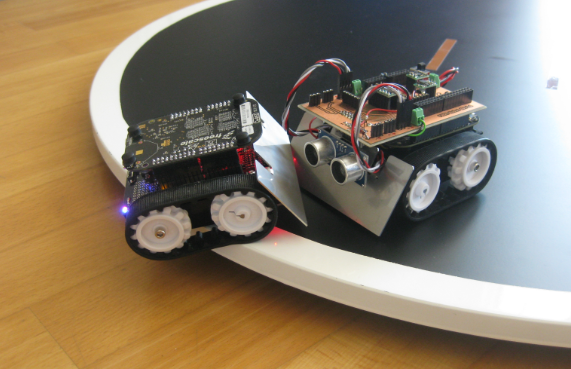
\includegraphics[height=6cm]{figures/sumo-robot-fight.png}

\section{Initial algorithm}
The simplest algorithm for a sumo robot is just randomly driving on the 
field, turning whenever we approach the field boundary:


\begin{lstlisting}
void loop(){
    readLineSensors();
    if (allOnBlack()){
        setMotors(70,70);//drive forward
    } else {
        //one of the sensors sees white
        goBackward(50);//back up 5 cm
        if (sensorOnWhite(DN1)) {
            //left sensor saw white
            turn(120); //turn 120 degrees right
        } else {
            //must have been the right sensor
            turn(-120);
        }
    }
}
\end{lstlisting}

Note that the sensor values used in ~if(sensorOnWhite(DN1))~ line are the values 
obtained at  last ~readLineSensors()~, which is before we back up. 


\section{Using proximity sensors}
A better algorithm, instead of blindly driving forward, would try to use 
front proximity sensors to detect the opponent. If we do see the opponent, 
we should go forward at full speed. If the opponent is not directly ahead 
but to a side, then we need to steer left or right as needed.

To make the program more readable, we use functions:

\begin{lstlisting}
void loop(){
    readLineSensors();
    if (allOnBlack()){
        lookForOpponent();
    } else {
        //one of the sensors sees white
        backFromEdge();
    }
}
\end{lstlisting}

Function ~backFromEdge()~ would be backing up from the edge and turning 
left/right as needed, using exactly the same code as before. Function
 ~lookForOpponent()~ should use the proximity sensors to check for opponent: 
\begin{lstlisting}
void lookForOpponent(){
    int left, right, correction;
    readProxSensors();
    left=proxSensorLevel(PROX_LF);
    right=proxSensorLevel(PROX_RF);
    if (left+right<3) {
        //very low signal -- no opponent nearby
        //let us just go forward 
        setMotors(70,70);
    } else {
        //we see opponnent!
         correction = 30.0*(left-right)/(left+right);
         setMotors(100-correction, 100+correction);
    }
}
\end{lstlisting}
One thing  worth commenting is how we determine the 
correction to the course. The general idea is similar to the one used 
in the line following algorithm: we use sensor feedback for correction. 
In this case, if left signal is stronger (thus, ~correction>0~), then 
we need to be turning left, i.e. left motor should get less power. 

We use the ratio $(l-r)/(l+r)$ as it is a better measure of difference 
of relative signal strengths. This expression ranges from $-1$ (if $l=0$, 
i.e. the signal only come from the right sensor) to $1$ (if the signal 
only comes from the left sensor). As before, you can experiment what happens if 
the coefficient of proportionality $30.0$ is replaced by a different value. 


\section{Advanced algorithm: using states}
The previous algorithm can be improved in several ways. For example, 
we could also use the side proximitye sensors: if one of them sees the 
opponnent, we need to turn to face it. Also, it seems a good idea that 
if we have been driving for some time without seeing the opponent,
we should stop driving and just turn in place, looking for the opponent. 

Trying to write such an agrorithm using the same ideas as before (basically 
as a series of ~if~ statements) is not easy and will result in a program 
which is very difficult to read --- and thus, easy to make a mistake. A better 
(and more common) apporach is to  introduce the idea of robot state:
at each moment, the robot can be in one of several states, or modes, such as 
``driving forward'', ``sweeping for opponent'', ``at edge'', etc. The behavior 
of the robot would not only depend on the current sensor readings, but also on 
its state. 

Thus, the outline of such a program would be 
\begin{lstlisting}
int state;
void loop(){
     ?set new state?
     ?move depending on the state and current sensors?
}
\end{lstlisting}

A suggested list of states is as follows:
\begin{itemize}
\item {\bf Driving}: we do not see an opponent and are just driving forward blindly. 
This is the default state.
\item {\bf At edge}: the robot is at the edge of the field
\item {\bf Opponent ahead}: we see an opponent ahead
\item {\bf Sweeping right}: robot is sweeping for opponent, by rotating clockwise
\item {\bf Sweeping left}: robot is sweeping for opponent, by rotating counterclockwise
\end{itemize}

For describing the state in the program, we could encode each state by an integer 
number (say, ~Driving =0~) and use these numbers in all our constructions: 
~if (state==0)...~. A better way is to use ~#define~ construction:
\begin{lstlisting}
#define DRIVING 0
#define AT_EDGE 1
...
int state;
...
if (state==DRIVING) {
...
}
\end{lstlisting}
Line ~#define DRIVING 0~ directs the computer to replace everywhere in the program 
word ~DRIVING~ by 0; essentially it defines an alias for the value 0. (Note that there is 
no equality sign in this construction, and no semicolon.) The benefit of this is that 
condition ~if (state==DRIVING) ~ is much easier to understand than ~if (state==0)~.

We now need to formulate the rules for state change: how the new state of the robot 
is determined? Generally, the new state will depend on the previous state and current values
of sensors. A reasonable choice of rules is as follows:

\begin{itemize}
\item If one of line sensors sees white, the state should be set to ~AT_EDGE~ 
    (regardless of the previous state)
\item Otherwise, if the front proximity sensors see opponent, the state should be 
set to\\ ~OPPONENT_AHEAD~ (regardless of previous state)
\item Otherwise, if the left/right proximity sensor sees opponent, the state should 
be set to ~SWEEP_LEFT~ or ~SWEEP_RIGHT~
\end{itemize}

These rules deal with immediate reaction to sensors. What about when the sensors 
do not see anything? 

\begin{itemize}
\item If the current state is ~DRIVING~ and we have been in this state long enough, 
set new state to ~SWEEP_LEFT~ (i.e., start looking for an opponent)
\item If the current state is ~SWEEP_LEFT~/~SWEEP_RIGHT~, and we have been in 
this state long enough, set the new state to ~DRIVING~; otherwise keep sweeping.
\item If none of the above rules apply, set the state to ~DRIVING~
\end{itemize}

The last rule is a general catch-all: it should deal, for example, with the situation 
when we were seeing the opponent ahead, and then it suddenly disappeared, or 
when we just backed up from the edge. 

To make precise  ``long enough'' used in the rules above, we could use motor encoders. 
For example, for driving, we could reset the encoders when we begin driving, and then 
use condition ~distanceTraveled()>2000~ instead of ``long enough'' (2000 mm=2 m). 

Similarly, for sweeping left/right, we could also reset the encoders once the sweep begins, 
and use ~abs(angleTurned())>360~ as the condiiton. 

Now that we have all these rules, we can program them. We will make a separate function 
~setState()~ that does this. 

\begin{lstlisting}
#define DRIVING 0
#define AT_EDGE 1
#define SWEEP_RIGHT 2
#define SWEEP_LEFT 3
#define OPPONENT_AHEAD 4
int state;
void setState(){
    readLineSensors();
    if (sensorOnWhite(DM1)||sensorOnWhite(DM5)) {
        state=AT_EDGE;
        return;
    }
    readProxSensors();
    if (proxSensorLevels(PROX_LF)+proxSensorLevels(PROX_RF)>3) {
        state=OPPONENT_AHEAD;
        return;     
    }
    if (proxSensorLevels(PROX_L)>1) {
        resetEncoders();
        state=SWEEP_LEFT;
        return;     
    }
    if (proxSensorLevels(PROX_R)>1) {
        resetEncoders();
        state=SWEEP_RIGHT;
        return;     
    }
    if (proxSensorLevels(PROX_LF)+proxSensorLevels(PROX_RF)>3) {
        state=OPPONENT_AHEAD;
        return;     
   }
   if (state==DRIVING) {
      if (distanceTraveled()>2000) {
          state=SWEEP_LEFT;
          resetEncoders();
      }
      //otherwise, do nothing - continue driving
      return;
   }
   if (state==SWEEP_LEFT || state==SWEEP_RIGHT){
      if (abs(angleTurned())>360) {
          state=DRIVING;
          resetEncoders();
      }
      //otherwise, do nothing - continue sweeping
      return;
   }
   //and finally, catch-all rule
   state=DRIVING;
   resetEncoders();
}
\end{lstlisting}

The main program would now look like this:
\begin{lstlisting}
void loop(){
    setState();
    switch (state) {
        case DRIVING:
            setMotors(70,70);
            break;
        case AT_EDGE:
            ...
            break;
        case SWEEP_LEFT:
            ...
            break;
        case SWEEP_RIGHT:
            ...
            break;
        case OPPONENT_AHEAD:
            ...
            break;
            
    }
}
\end{lstlisting}
The code for setting robot motion in  ~OPPONENT_AHEAD~ state should be steering 
left/right, using the values of two front proximity sensors for feedback, as was done 
in the previous section.

%%%%%%%%%%%%%%%%%%%%%
\chapter{Appendix A: Arduino basics}\label{c:arduino}
\section{Basic program structure}
\par\noindent
\begin{lstlisting}
void setup() {
  // put your setup code here, to run once:

}

void loop() {
  // put your main code here, to run repeatedly: 
  
}
\end{lstlisting}

\subsection*{Comments}
Single-line comment: everything from ~//~ to end of line.

Multi-line comment: everything between ~/*~ and ~*/~:
\begin{lstlisting}
 x=x+1; //this is a single line comment
 /*  and this is a 
   multi-line comment */
  
\end{lstlisting}

\subsection*{Control structures}
\par\noindent
\begin{lstlisting}
// if statements
if (?condition?) {
 ...
} else {
 ...
}
//while loops
while(?condition?){
...
}
\end{lstlisting}

\subsection*{Logical operators}
Used to construct conditions: 

Comparison: ~==~ (e.g., ~if (x==5) {.. }~). 


AND: ~&&~

OR: ~||~ 

NOT: ~!~ 

\begin{lstlisting}

while (time<1000 && !sensorOnWhite()){
...
}
  
\end{lstlisting}

\begin{warning}
When comparing two values, make sure you use ~==~ rather than ~=~. 
A common beginners mistake is writing something like ~if (x=5)~. Instead 
of checking whether ~x~ is equal to 5, this will {\bf assign} to ~x~ value 5  
(and will give ~true~ logical value). 
\end{warning}


\section{Variables and constants}\par\noindent

Variable declaration:
\begin{lstlisting}
    int n=10;
\end{lstlisting}
Usually these declarations are placed in the beginnign of the file, before ~void setup()~.

Basic variable types: ~int~, ~long~ (long integer, gives larger range), ~float~, ~boolean~, ~String~ (note
uppercase!). 

Constant declarations: 
\begin{lstlisting}
    constant int CUTOFF=40;
\end{lstlisting}

Pre-defined boolean constants: ~true~, ~false~. 
\subsection*{Strings}
Defining a string: ~String s="Hello World!";~

(note the double quotes).

Turning numbers into strings: 
\begin{lstlisting}
float x=5.17
String s=String(x);
\end{lstlisting}

Concatenating (putting together) strings:
\begin{lstlisting}
String s="x="+String(x);
\end{lstlisting}

\section{Functions}
\subsection*{Some standard functions}
\ 
\par\noindent
\begin{tabular}{|l | l | p{7cm} |}
\hline 
~int~ & ~abs(int x)~& Absolute value. Instead of ~int~, can also use
~float~\\
\hline 
~int~ & ~max(int x, int y)~ & Maximum of two numbers. Instead of ~int~, can
also use
~float~\\
\hline
~long~ & ~millis()~ & Number of milliseconds since the program started\\
\hline
~void~ & ~delay(unsigned long ms)~ & Pause program executions for specified number of millisecons\\
\hline

\end{tabular}

\subsection*{Defining your own functions}

To define your own function, you need to declare it as shown below:
\begin{lstlisting}
int myFunction(int a, int b){
  ?body of the function?
}
\end{lstlisting}

This declaration can be placed in any place in the file (but not 
inside other functions); usually it is placed after the end of ~loop()~. 

The first word (in this case ~int~) is the type of the value returned by the 
function. If your function does not return any values, use ~void~. 

~myFunction~ is the name of the function; it must satisfy the usual properties 
(can only contain letters, digits, and underscore, and can not coincide with existing 
variable and function names).

After function name, you put in parentheses the arguments, or inputs to the 
function. In this case, there are two arguments, both of type ~int~. If your 
function does not have any arguments, put nothing between the parentheses: 
~myFunction()~. 

Inside the body of the function, you can put any code. You can also use global 
variables (those defined in the beginning of the program, outside of any 
functions) and arguments (such as ~a~, ~b~ in the example above). You can 
also introduce new variables, called local variables; these variables will only be 
accessible inside the function, and their values are not saved once the function 
execution completes: if the same fucntion is called again, the values of local 
variables are initialized again. 

To finish the function and return a value, use ~return(value);~. 

Below is an example of a function, which computes the factorial of a number: 
$n!=1\cdot 2\cdots \cdots n$.
 \begin{lstlisting}
 int factorial(int n){
     int f=1;
     int i=1;
     if (n<0) { //invalid input!
         return(0);
     }
     while (i<=n) {
         f=f*i;
         i=i+1;
     }
     return(f);
 }
 \end{lstlisting}

\end{document}
